\documentclass{article}
\usepackage[utf8]{inputenc}
\usepackage{graphicx}
\usepackage{booktabs}
\usepackage{longtable}
\usepackage{geometry}
\geometry{legalpaper}
\usepackage{standalone}

\title{Distribusi Poisson}
\date{}
\author{}

\begin{document}

	\maketitle
	
	\section{Tujuan}
		1. Mempelajari karakteristik statistik peluruhan radioaktif.\\
		2. Menentukan aktivitas peluruhan preparat radioaktif.
	
	\section{Dasar Teori}
	 
		\hspace{0.35 cm} Radioaktif adalah suatu atom yang tidak stabil yang selalu melepaskan energi dan atau partikel untuk mencapai kestabilan di dalam inti atomnya\cite{modul}. Proses pelepasan energi radiasi atau partikel ini dikenal dengan istilah peluruhan. Walaupun proses peluruhan ini bersifat acak, namun apabila jumlah partikel yang dilepaskan dalam selang waktu tertentu ternyata memiliki pola kecenderungan tertentu secara statistik.\par
		Kemungkinan suatu preparat radioaktif akan meluruh dengan melepaskan $n$ partikel dalam selang waktu $\Delta t$ tertentu dapat diperkirakan melalui pendekatan distribusi Poisson 
		sebagai berikut: 
		\begin{equation}
		W_{\mu}(n) = \frac{\mu^n}{n!}\cdot e^{-\mu}
		\end{equation}
		dimana:
		\par $W_{\mu}(n)$: probabilitas peluruhan $n$ partikel
		\par $\mu$: nilai rata-rata peluruhan
		\par $n$: jumlah partikel yang meluruh \\
		
		\par Secara teoritis nilai $\mu$ sangat dipengaruhi oleh ukuran preparat dan selang waktu $\Delta t$, serta berbanding terbalik dengan waktu paruh $T_{1/2}$ dari radioaktif tersebut\cite{modul}. 
	
		
		
		\begin{center}
			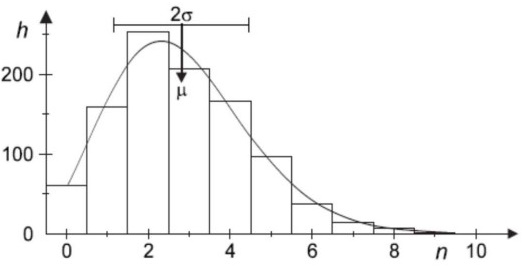
\includegraphics[width=110mm]{Picture/1.jpg}\\
			Gambar 1. Distribusi Poisson hasil pengukuran dan perhitungan. \\ Histogram: $h(n)$ dan kurva: $N.W_{\mu}$
		\end{center}
		
		\par Standard deviasi atau simpangan baku untuk distribusi Poisson dapat dihitung dengan persamaan berikut: 
		
		\begin{equation}
			\sigma = \sqrt{\mu}
		\end{equation}
	
	\section{Peralatan}
	1. 1 Unit komputer terkoneksi internet \\
	2. 1 Unit sistem kontrol \\ 
	3. 1 Set preparat radioaktif \\
	4. 1 Pencacah Geiger Muller \\
	5. 1 Sensor Cassy \\
	6. 1 GM Box 
	
	\section{Metode Eksperimen}
	
		\hspace{0.35 cm} Pada eksperimen ini, akan dihitung frekuensi dari sejumlah $n$ partikel yang meluruh dalam selang waktu $\Delta t$ tertentu. Pengukuran tersebut dilakukan terhadap 5 jenis preparat radioaktif yang berbeda yang dihitung dengan menggunakan pencacah Geiger Muller. Setiap preparat akan dilakukan pengambilan data sebanyak $500$ data yang selanjutnya dapat ditampilkan dalam bentuk histogram. 
		
		\par Berdasarkan data tersebut, akan dihitung nilai rata-rata peluruhan $\mu$ dan simpangan bakunya $\sigma$ dengan pendekatan distribusi Poisson. Untuk preparat yang memiliki nilai rata-rata $\mu$ yang besar, dilakukan pula pendekatan distribusi normal atau Gausssian sebagai pembanding untuk membuktikan pola distribusi yang paling sesuai. 
	
	\section{Pengolahan Data}
		
		\begin{equation}
		w = \frac{h}{i}
		\end{equation}
		dengan:\\
		$w$ = nilai probabilitas distribusi Poisson ternormalisasi\\
		$i$ = jumlah data (500 data)\\
		$h$ = nilai frekuensi pada histogram\\ \\
		kemudian, mengolah data menggunakan regresi linier dengan persamaan:
		\begin{equation}
		ln(w.n!) = ln(\mu).n-\mu
		\end{equation}
		\begin{equation}
		y = bx+a
		\end{equation}
		dan, standar deviasinya adalah:\\
		\begin{equation}
		\sigma = \sqrt{\mu} = \sqrt{-a}
		\end{equation}
			
			\subsection{Na-22}
			Tabel Pengolahan Data:
			
			\begin{longtable}{@{}lllllllll@{}} 
					\toprule
					No  & $n$  & $n^{2}$ & $n!$   & $h$   & $w$     & $ln(w.n!)$     & $ln^{2}(w.n!)$ & $n.ln(w.n!)$   \\ \midrule
				\endfirsthead
				%
				\endhead
				%
				\bottomrule
				\endfoot
				%
				\endlastfoot
				%
				1   & 0  & 0                    & 1    & 85  & 0.17  & -1.771956842 & 3.13983105                  & 0            \\
				2   & 1  & 1                    & 1    & 155 & 0.31  & -1.171182982 & 1.371669576                 & -1.171182982 \\
				3   & 2  & 4                    & 2    & 136 & 0.272 & -0.608806032 & 0.370644785                 & -1.217612064 \\
				4   & 3  & 9                    & 6    & 77  & 0.154 & -0.079043207 & 0.006247829                 & -0.237129622 \\
				5   & 4  & 16                   & 24   & 31  & 0.062 & 0.397432936  & 0.157952939                 & 1.589731746  \\
				6   & 5  & 25                   & 120  & 10  & 0.02  & 0.875468737  & 0.76644551                  & 4.377343687  \\
				7   & 6  & 36                   & 720  & 5   & 0.01  & 1.974081026  & 3.896995897                 & 11.84448616  \\
				8   & 7  & 49                   & 5040 & 1   & 0.002 & 2.310553263  & 5.33865638                  & 16.17387284  \\* \midrule
				$\Sigma$ & 28 & 140                  & 5914 & 500 & 1     & 1.926546899  & 15.04844397                 & 31.35950977  \\* \bottomrule
				\end{longtable} \newpage
			\hspace{-0.6cm}Koefisien Regresi, \\
			$a = -1.81056461$ \\
			$b = 0.58610942$ \\ \\
			Error,\\
			$r^{2} = 0.9892709672063679$ \\
			$r = 0.9946210168734461 $ \\ \\
			Grafik: 
			\begin{center}
				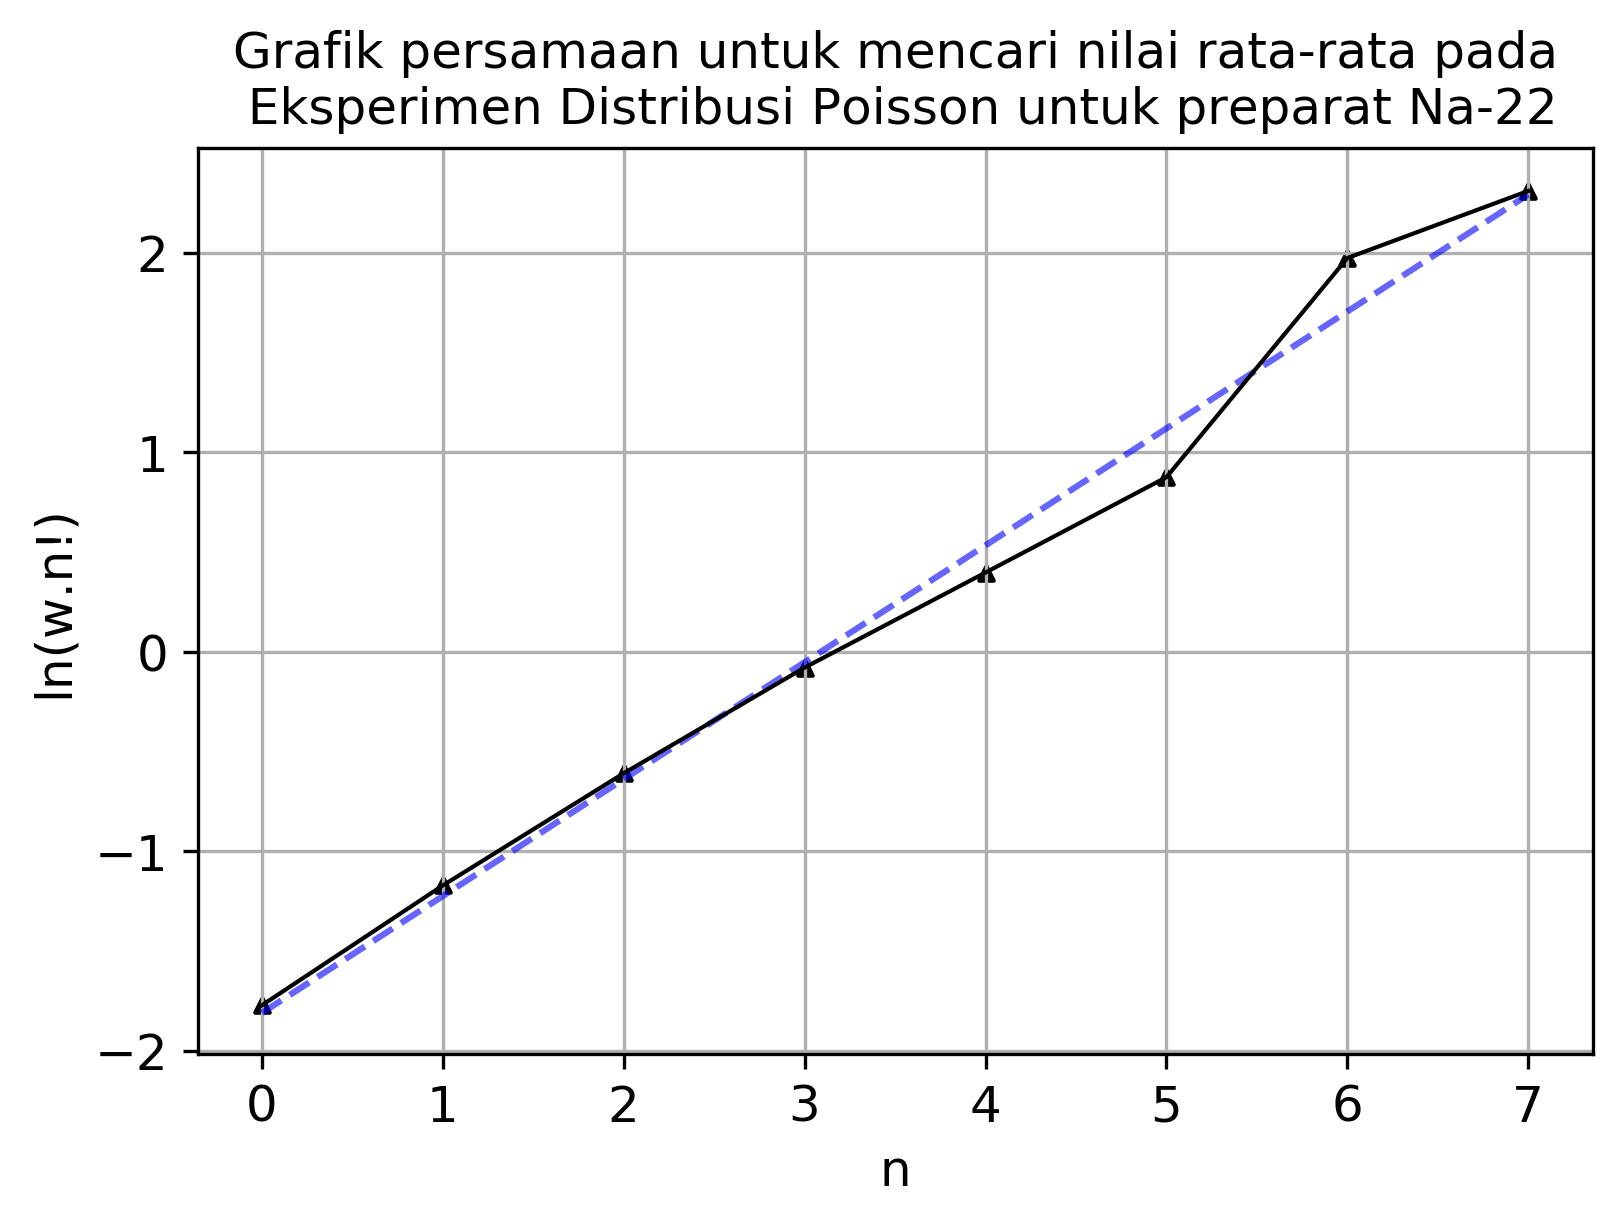
\includegraphics[width=110mm]{Data/Na-22-Graph.png}\\
				Gambar 2. Grafik Regresi Linier dari Preparat Na-22.
			\end{center}
			Grafik Histogram:
			\begin{center}
				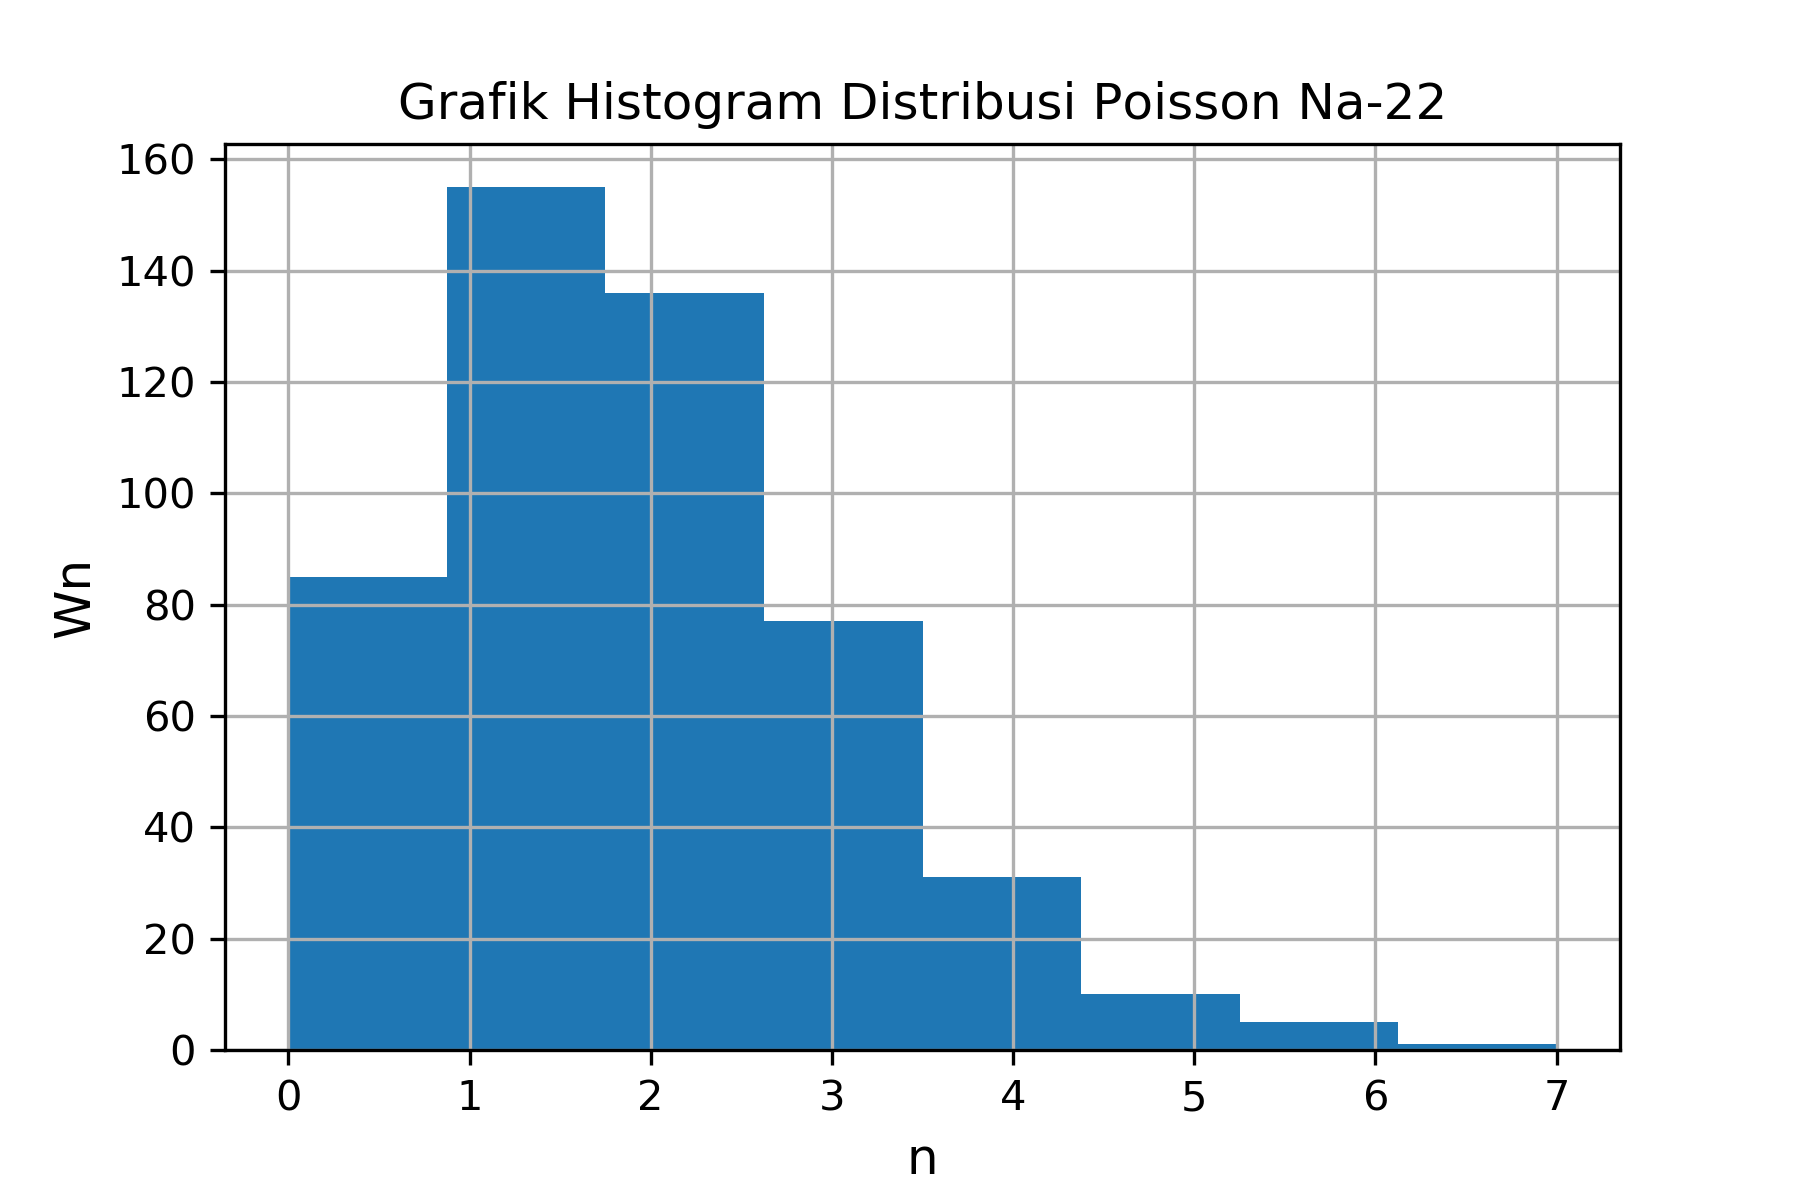
\includegraphics[width=110mm]{Data/Na-22.png}\\
				Gambar 3. Grafik Histogram dari Preparat Na-22.
			\end{center}
			Nilai rata-rata standar deviasi $\sigma = \sqrt{\mu}$ berdasarkan histogram:\\
			$\sigma = \sqrt{-(-1.81056461)} = 1.345572223999886$ \newpage
			
			\subsection{Co-60}
			Tabel Pengolahan Data: 
			\begin{longtable}{@{}lllllllll@{}}
				\toprule
				No  & $n$  & $n^{2}$ & $n!$   & $h$   & $w$     & $ln(w.n!)$     & $ln^{2}(w.n!)$ & $n.ln(w.n!)$   \\ \midrule
				\endfirsthead
				%
				\endhead
				%
				\bottomrule
				\endfoot
				%
				\endlastfoot
				%
				1   & 0  & 0                    & 1   & 129 & 0.258 & -1.354795694 & 1.835471373                 & 0            \\
				2   & 1  & 1                    & 1   & 169 & 0.338 & -1.084709383 & 1.176594447                 & -1.084709383 \\
				3   & 2  & 4                    & 2   & 127 & 0.254 & -0.677273831 & 0.458699843                 & -1.354547663 \\
				4   & 3  & 9                    & 6   & 55  & 0.11  & -0.415515444 & 0.172653084                 & -1.246546332 \\
				5   & 4  & 16                   & 24  & 12  & 0.024 & -0.551647618 & 0.304315095                 & -2.206590473 \\
				6   & 5  & 25                   & 120 & 7   & 0.014 & 0.518793793  & 0.269147                    & 2.593968967  \\
				7   & 6  & 36                   & 720 & 1   & 0.002 & 0.364643114  & 0.1329646                   & 2.187858682  \\* \midrule
				$\Sigma$ & 21 & 91                   & 874 & 500 & 1     & -3.200505063 & 4.349845442                 & -1.110566202 \\* \bottomrule
			\end{longtable}
			\hspace{-0.6cm}Koefisien Regresi, \\
			$a = -1.36695954$ \\
			$b = 0.30324818$ \\ \\
			Error,\\
			$r^{2} = 0.8920288182711459$ \\
			$r = 0.9444727726468063$ \\ \\
			Grafik: 
			\begin{center}
				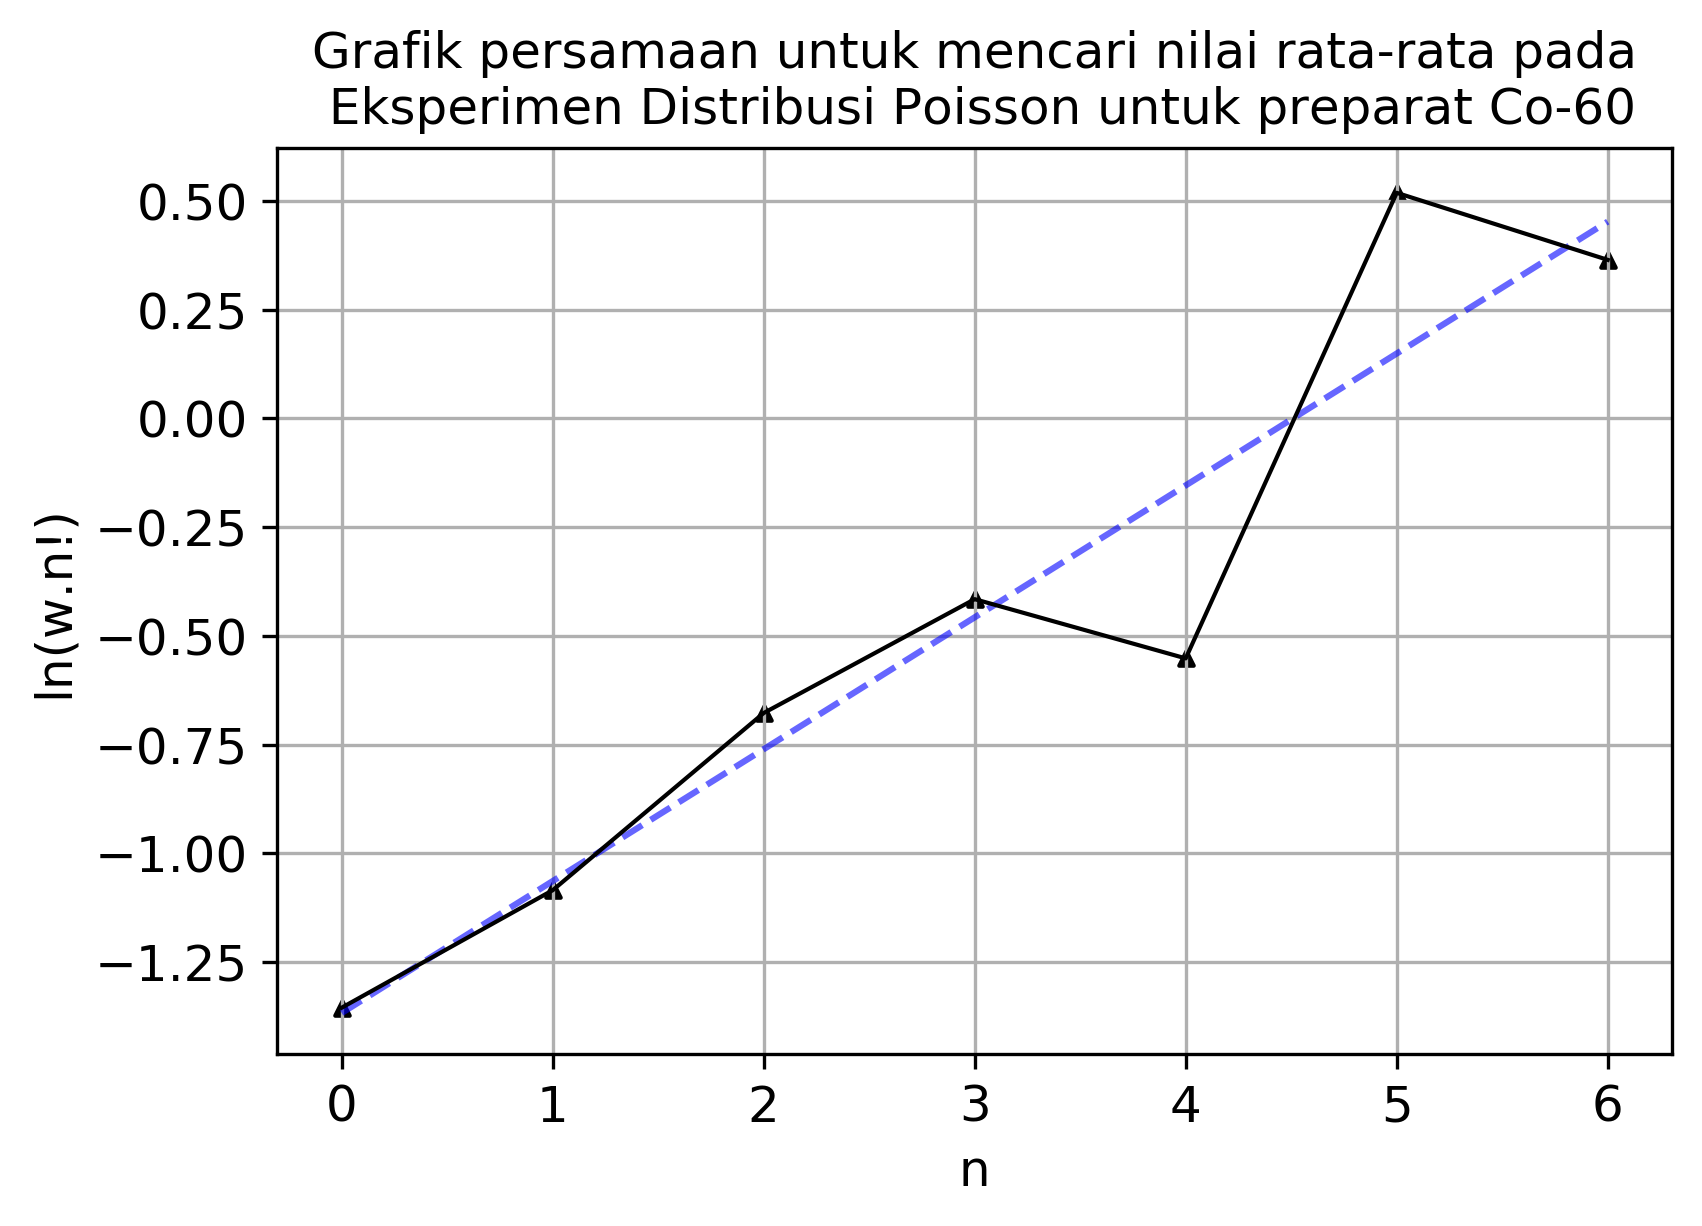
\includegraphics[width=110mm]{Data/Co-60-Graph.png}\\
				Gambar 4. Grafik Regresi Linier dari Preparat Co-60.
			\end{center}\newpage
			Grafik Histogram:
			\begin{center}
				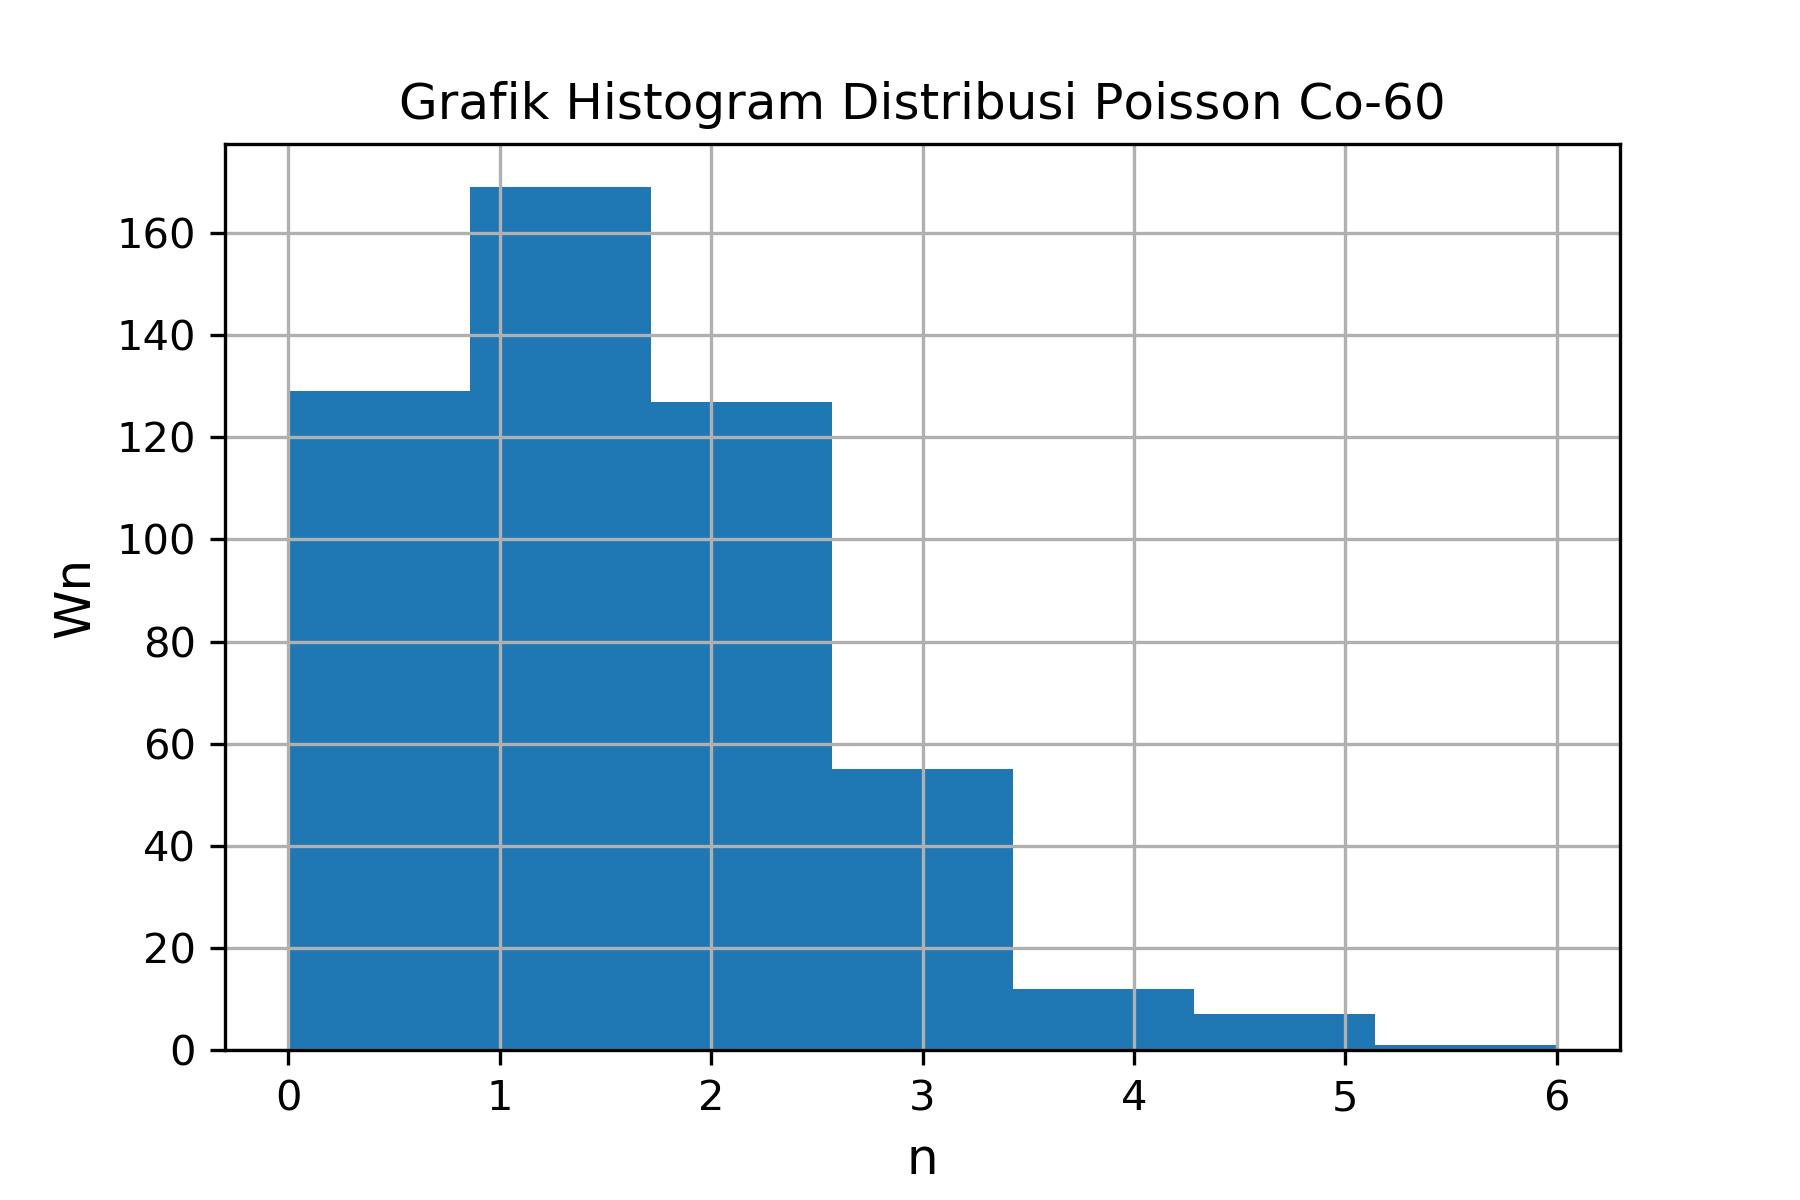
\includegraphics[width=110mm]{Data/Co-60.png}\\
				Gambar 5. Grafik Histogram dari Preparat Co-60.
			\end{center} 
			Nilai rata-rata standar deviasi $\sigma = \sqrt{\mu}$ berdasarkan histogram:\\
			$\sigma = \sqrt{-(-1.36695954)} = 1.169170449506829$ 		
			
			\subsection{Sr-90}
			Tabel Pengolahan Data:
			\begin{longtable}{@{}lllllllll@{}}
				\toprule
				No  & $n$  & $n^{2}$ & $n!$   & $h$   & $w$     & $ln(w.n!)$     & $ln^{2}(w.n!)$ & $n.ln(w.n!)$   \\ \midrule
				\endfirsthead
				%
				\endhead
				%
				\bottomrule
				\endfoot
				%
				\endlastfoot
				%
				1   & 40   & 1600                 & 8.16E+47    & 2   & 0.004 & 104.7991788 & 10982.86788                 & 4191.967152 \\
				2   & 42   & 1764                 & 1.41E+51    & 3   & 0.006 & 112.6558856 & 12691.34856                 & 4731.547195 \\
				3   & 43   & 1849                 & 6.04E+52    & 2   & 0.004 & 116.0116206 & 13458.69611                 & 4988.499686 \\
				4   & 45   & 2025                 & 1.20E+56    & 3   & 0.006 & 124.0079378 & 15377.96864                 & 5580.357202 \\
				5   & 46   & 2116                 & 5.50E+57    & 1   & 0.002 & 126.7379669 & 16062.51226                 & 5829.946479 \\
				6   & 47   & 2209                 & 2.59E+59    & 5   & 0.01  & 132.1975525 & 17476.19287                 & 6213.284965 \\
				7   & 48   & 2304                 & 1.24E+61    & 2   & 0.004 & 135.1524627 & 18266.18818                 & 6487.318211 \\
				8   & 49   & 2401                 & 6.08E+62    & 11  & 0.022 & 140.7490311 & 19810.28976                 & 6896.702525 \\
				9   & 50   & 2500                 & 3.04E+64    & 8   & 0.016 & 144.3426004 & 20834.78629                 & 7217.13002  \\
				10  & 51   & 2601                 & 1.55E+66    & 8   & 0.016 & 148.274426  & 21985.30541                 & 7561.995727 \\
				11  & 52   & 2704                 & 8.07E+67    & 7   & 0.014 & 152.0921384 & 23132.01855                 & 7908.791194 \\
				12  & 53   & 2809                 & 4.27E+69    & 9   & 0.018 & 156.3137447 & 24433.98678                 & 8284.628469 \\
				13  & 54   & 2916                 & 2.31E+71    & 16  & 0.032 & 160.8780929 & 25881.76077                 & 8687.417016 \\
				14  & 55   & 3025                 & 1.27E+73    & 25  & 0.05  & 165.3317132 & 27334.57538                 & 9093.244225 \\
				15  & 56   & 3136                 & 7.11E+74    & 16  & 0.032 & 168.9107778 & 28530.85084                 & 9459.003555 \\
				16  & 57   & 3249                 & 4.05E+76    & 25  & 0.05  & 173.4001161 & 30067.60028                 & 9883.80662  \\
				17  & 58   & 3364                 & 2.35E+78    & 22  & 0.044 & 177.3327258 & 31446.89563                 & 10285.29809 \\
				18  & 59   & 3481                 & 1.39E+80    & 32  & 0.064 & 181.7849567 & 33045.77047                 & 10725.31244 \\
				19  & 60   & 3600                 & 8.32E+81    & 16  & 0.032 & 185.186154  & 34293.91165                 & 11111.16924 \\
				20  & 61   & 3721                 & 5.08E+83    & 23  & 0.046 & 189.6599334 & 35970.89034                 & 11569.25594 \\
				21  & 62   & 3844                 & 3.15E+85    & 21  & 0.042 & 193.696096  & 37518.17761                 & 12009.15795 \\
				22  & 63   & 3969                 & 1.98E+87    & 31  & 0.062 & 198.2286955 & 39294.61572                 & 12488.40782 \\
				23  & 64   & 4096                 & 1.27E+89    & 25  & 0.05  & 202.1724672 & 40873.7065                  & 12939.0379  \\
				24  & 65   & 4225                 & 8.25E+90    & 21  & 0.042 & 206.1725011 & 42507.10021                 & 13401.21257 \\
				25  & 66   & 4356                 & 5.44E+92    & 25  & 0.05  & 210.5365092 & 44325.62171                 & 13895.40961 \\
				26  & 67   & 4489                 & 3.65E+94    & 17  & 0.034 & 214.3555394 & 45948.29725                 & 14361.82114 \\
				27  & 68   & 4624                 & 2.48E+96    & 16  & 0.032 & 218.5144224 & 47748.55282                 & 14858.98073 \\
				28  & 69   & 4761                 & 1.71E+98    & 16  & 0.032 & 222.7485289 & 49616.90715                 & 15369.6485  \\
				29  & 70   & 4900                 & 1.20E+100   & 17  & 0.034 & 227.0576488 & 51555.17588                 & 15894.03542 \\
				30  & 71   & 5041                 & 8.50E+101   & 13  & 0.026 & 231.0520647 & 53385.0566                  & 16404.69659 \\
				31  & 72   & 5184                 & 6.12E+103   & 12  & 0.024 & 235.2486881 & 55341.94526                 & 16937.90554 \\
				32  & 73   & 5329                 & 4.47E+105   & 5   & 0.01  & 238.6636788 & 56960.35159                 & 17422.44855 \\
				33  & 74   & 5476                 & 3.31E+107   & 7   & 0.014 & 243.3042161 & 59196.94159                 & 18004.51199 \\
				34  & 75   & 5625                 & 2.48E+109   & 6   & 0.012 & 247.4675536 & 61240.19008                 & 18560.06652 \\
				35  & 76   & 5776                 & 1.89E+111   & 8   & 0.016 & 252.085969  & 63547.33576                 & 19158.53364 \\
				36  & 77   & 5929                 & 1.45E+113   & 8   & 0.016 & 256.4297744 & 65756.22921                 & 19745.09263 \\
				37  & 78   & 6084                 & 1.13E+115   & 2   & 0.004 & 259.4001889 & 67288.45799                 & 20233.21473 \\
				38  & 79   & 6241                 & 8.95E+116   & 7   & 0.014 & 265.0223997 & 70236.87234                 & 20936.76958 \\
				39  & 80   & 6400                 & 7.16E+118   & 1   & 0.002 & 267.4585162 & 71534.05788                 & 21396.68129 \\
				40  & 81   & 6561                 & 5.80E+120   & 3   & 0.006 & 272.9515776 & 74502.56373                 & 22109.07779 \\
				41  & 82   & 6724                 & 4.75E+122   & 1   & 0.002 & 276.2596846 & 76319.41333                 & 22653.29414 \\
				42  & 83   & 6889                 & 3.95E+124   & 2   & 0.004 & 281.3716724 & 79170.01802                 & 23353.84881 \\* \midrule
				$\Sigma$ & 2621 & 169897               & 3.9981E+124 & 500 & 1     & 8216.017408 & 1714952.005                 & 538840.5294 \\* \bottomrule
			\end{longtable}
			\hspace{-0.6cm}Koefisien Regresi, \\
			$a = -61.73789708$ \\
			$b =4.12400194 $ \\ \\
			Error,\\
			$r^{2} = 0.9998862687766302$ \\
			$r = 0.9999431327713743$ \\ \\
			Grafik: 
			\begin{center}
				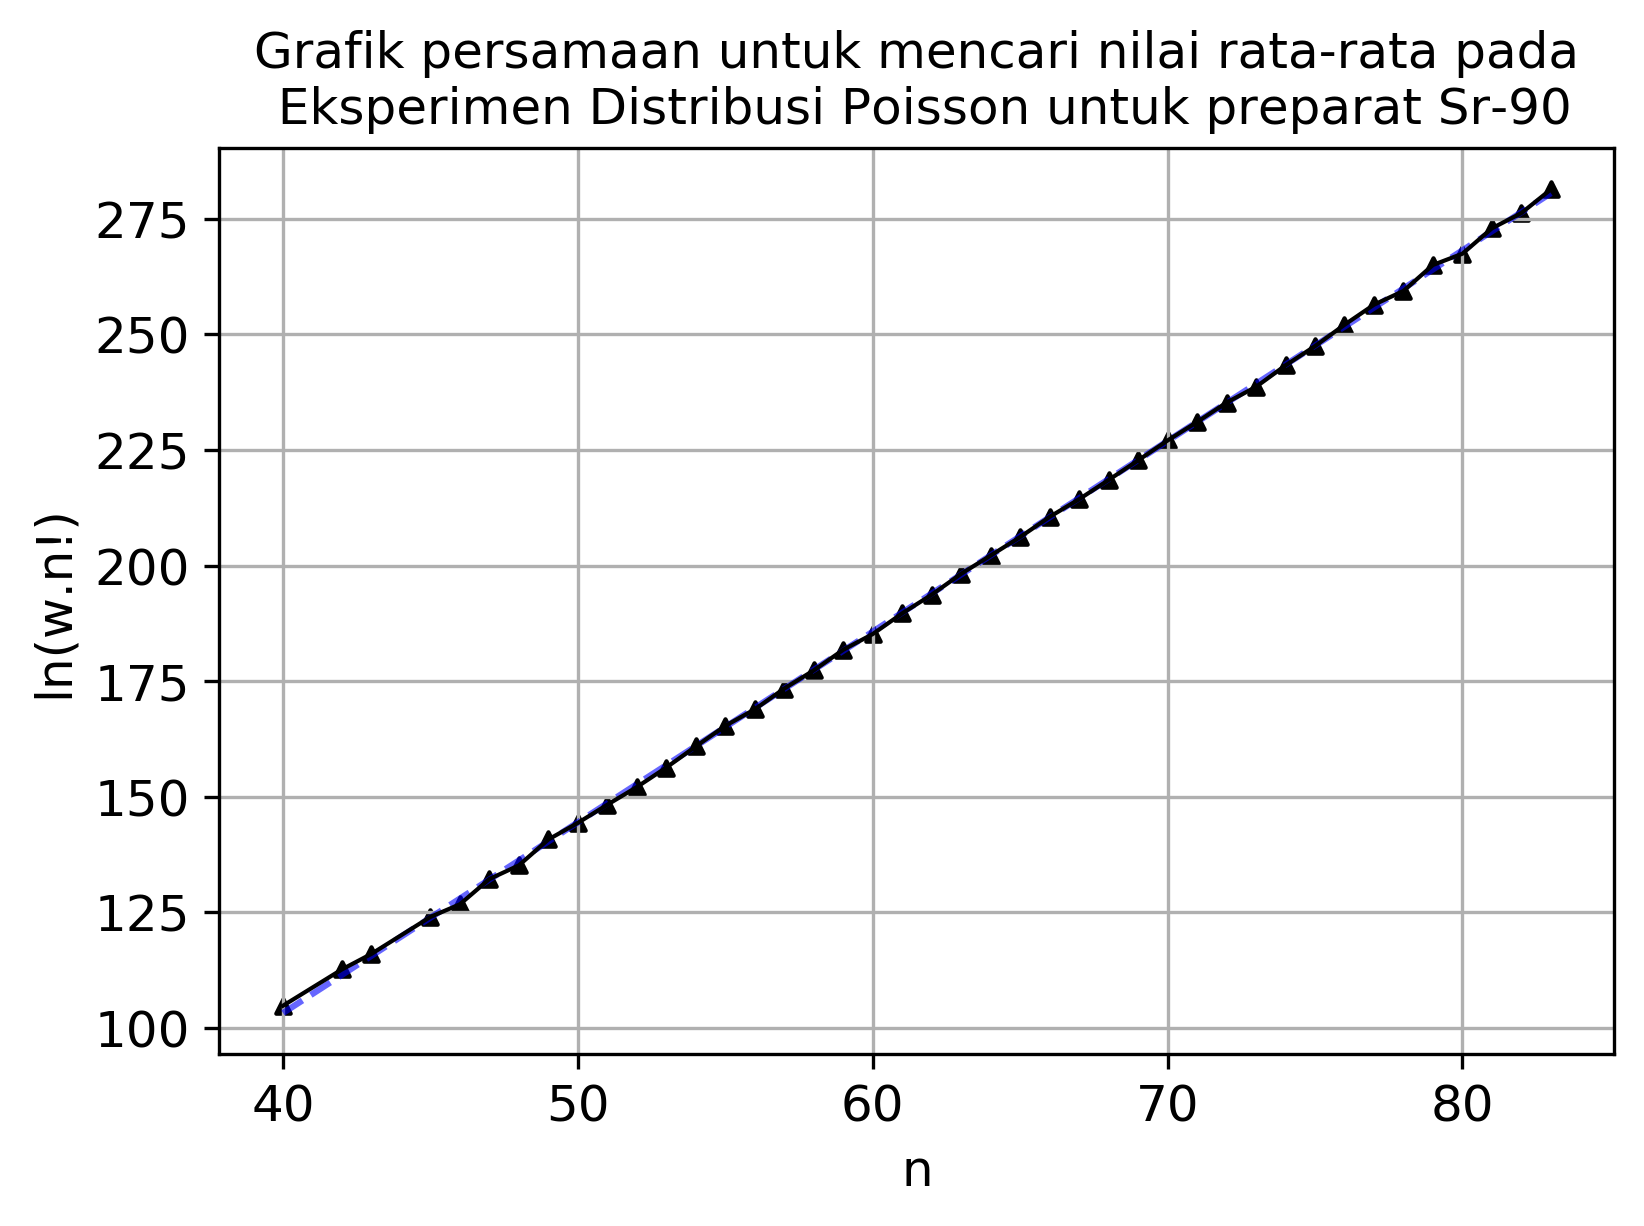
\includegraphics[width=110mm]{Data/Sr-90-Graph.png}\\
				Gambar 6. Grafik Regresi Linier dari Preparat Sr-90.
			\end{center}\newpage
			Grafik Histogram:
			\begin{center}
				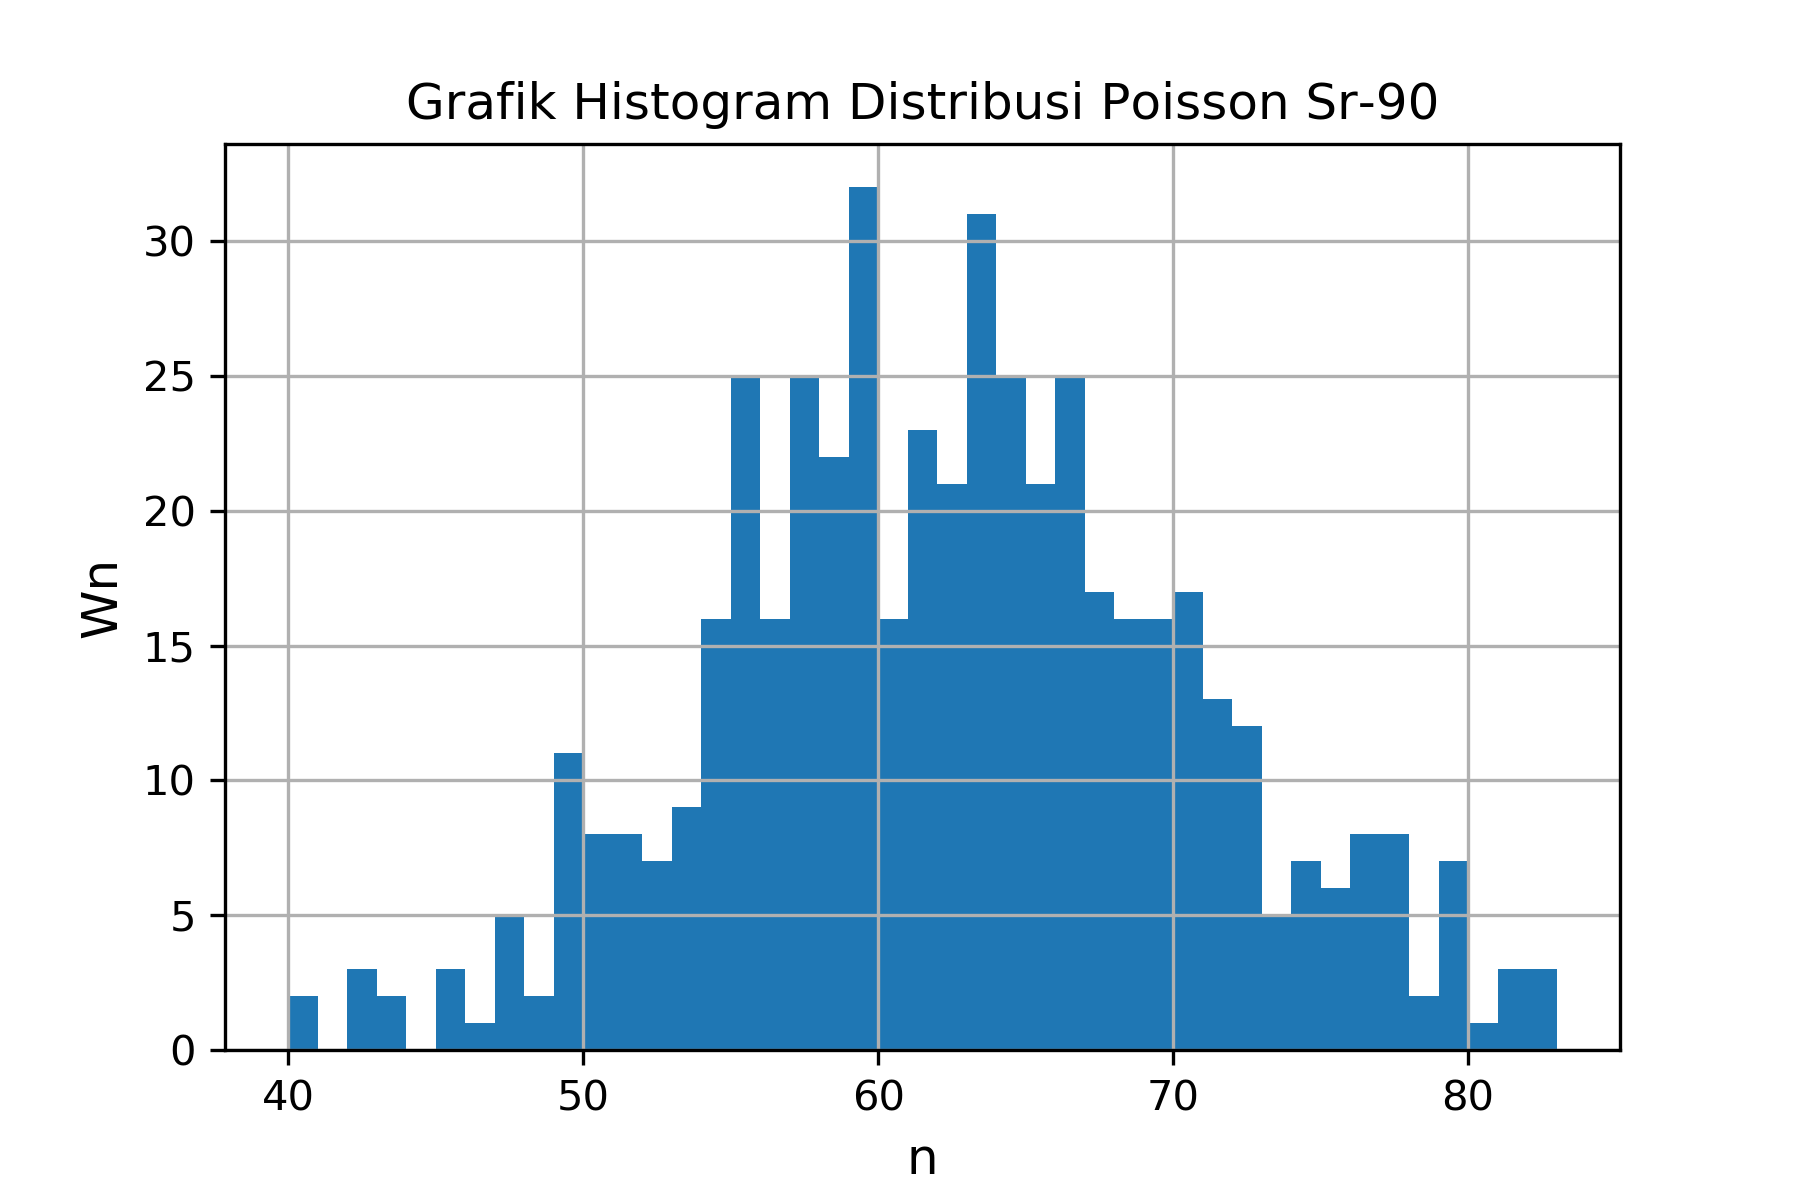
\includegraphics[width=110mm]{Data/Sr-90.png}\\
				Gambar 7. Grafik Histogram dari Preparat Sr-90.
			\end{center} 
			Nilai rata-rata standar deviasi $\sigma = \sqrt{\mu}$ berdasarkan histogram:\\
			$\sigma = \sqrt{-(-61.73789708)} = 7.857346694654627$
				
			\subsection{Cs-137}
			Tabel Pengolahan Data:
			\begin{longtable}{@{}lllllllll@{}}
				\toprule
				No  & $n$  & $n^{2}$ & $n!$   & $h$   & $w$     & $ln(w.n!)$     & $ln^{2}(w.n!)$ & $n.ln(w.n!)$   \\ \midrule
				\endfirsthead
				%
				\endhead
				%
				\bottomrule
				\endfoot
				%
				\endlastfoot
				%
				1   & 0   & 0                    & 1           & 2   & 0.004 & -5.521460918 & 30.48653067                 & 0            \\
				2   & 1   & 1                    & 1           & 5   & 0.01  & -4.605170186 & 21.20759244                 & -4.605170186 \\
				3   & 2   & 4                    & 2           & 17  & 0.034 & -2.688247574 & 7.226675018                 & -5.376495148 \\
				4   & 3   & 9                    & 6           & 33  & 0.066 & -0.926341068 & 0.858107774                 & -2.779023203 \\
				5   & 4   & 16                   & 24          & 59  & 0.118 & 1.040983176  & 1.083645972                 & 4.163932703  \\
				6   & 5   & 25                   & 120         & 92  & 0.184 & 3.094672221  & 9.576996158                 & 15.47336111  \\
				7   & 6   & 36                   & 720         & 95  & 0.19  & 4.918520005  & 24.19183904                 & 29.51112003  \\
				8   & 7   & 49                   & 5040        & 65  & 0.13  & 6.484940533  & 42.05445371                 & 45.39458373  \\
				9   & 8   & 64                   & 40320       & 54  & 0.108 & 8.378978851  & 70.20728658                 & 67.03183081  \\
				10  & 9   & 81                   & 362880      & 27  & 0.054 & 9.883056248  & 97.67480079                 & 88.94750623  \\
				11  & 10  & 100                  & 3628800     & 19  & 0.038 & 11.83424345  & 140.0493181                 & 118.3424345  \\
				12  & 11  & 121                  & 39916800    & 24  & 0.048 & 14.46575358  & 209.2580266                 & 159.1232894  \\
				13  & 12  & 144                  & 479001600   & 3   & 0.006 & 14.87121869  & 221.1531452                 & 178.4546242  \\
				14  & 13  & 169                  & 6227020800  & 3   & 0.006 & 17.43616804  & 304.019956                  & 226.6701846  \\
				15  & 14  & 196                  & 87178291200 & 1   & 0.002 & 18.97661308  & 360.1118442                 & 265.6725832  \\
				16  & 15  & 225                  & 1.31E+12    & 1   & 0.002 & 21.68466329  & 470.2246218                 & 325.2699493  \\* \midrule
				$\Sigma$ & 120 & 1240                 & 1.40393E+12 & 500 & 1     & 119.3285914  & 2009.38484                  & 1511.294711  \\* \bottomrule
			\end{longtable}
			\hspace{-0.6cm}Koefisien Regresi, \\
			$a = -6.13748382$ \\
			$b = 1.8127361$ \\ \\
			Error,\\
			$r^{2} = 0.9980493145499695$ \\
			$r = 0.9990241811637842$ \\ \newpage
			Grafik: 
			\begin{center}
				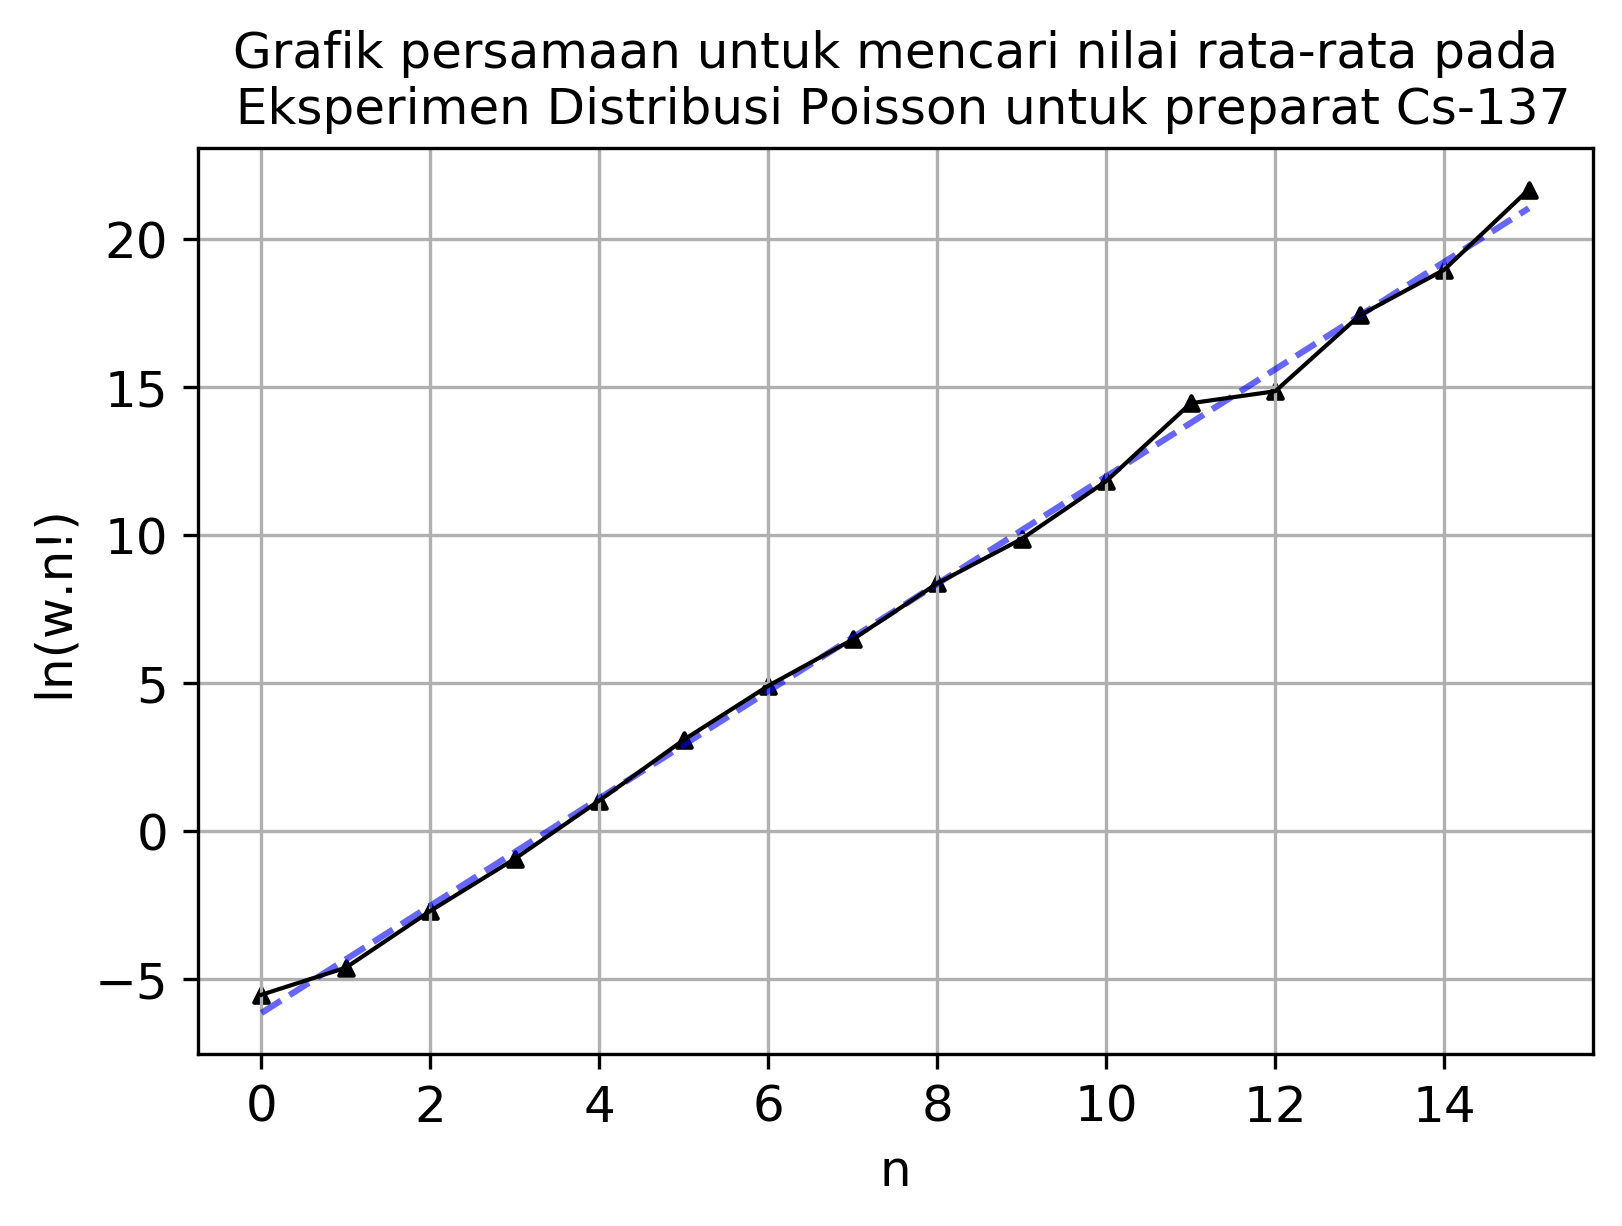
\includegraphics[width=110mm]{Data/Cs-137-Graph.png}\\
				Gambar 8. Grafik Regresi Linier dari Preparat Cs-137.
			\end{center}
			Grafik Histogram:
			\begin{center}
				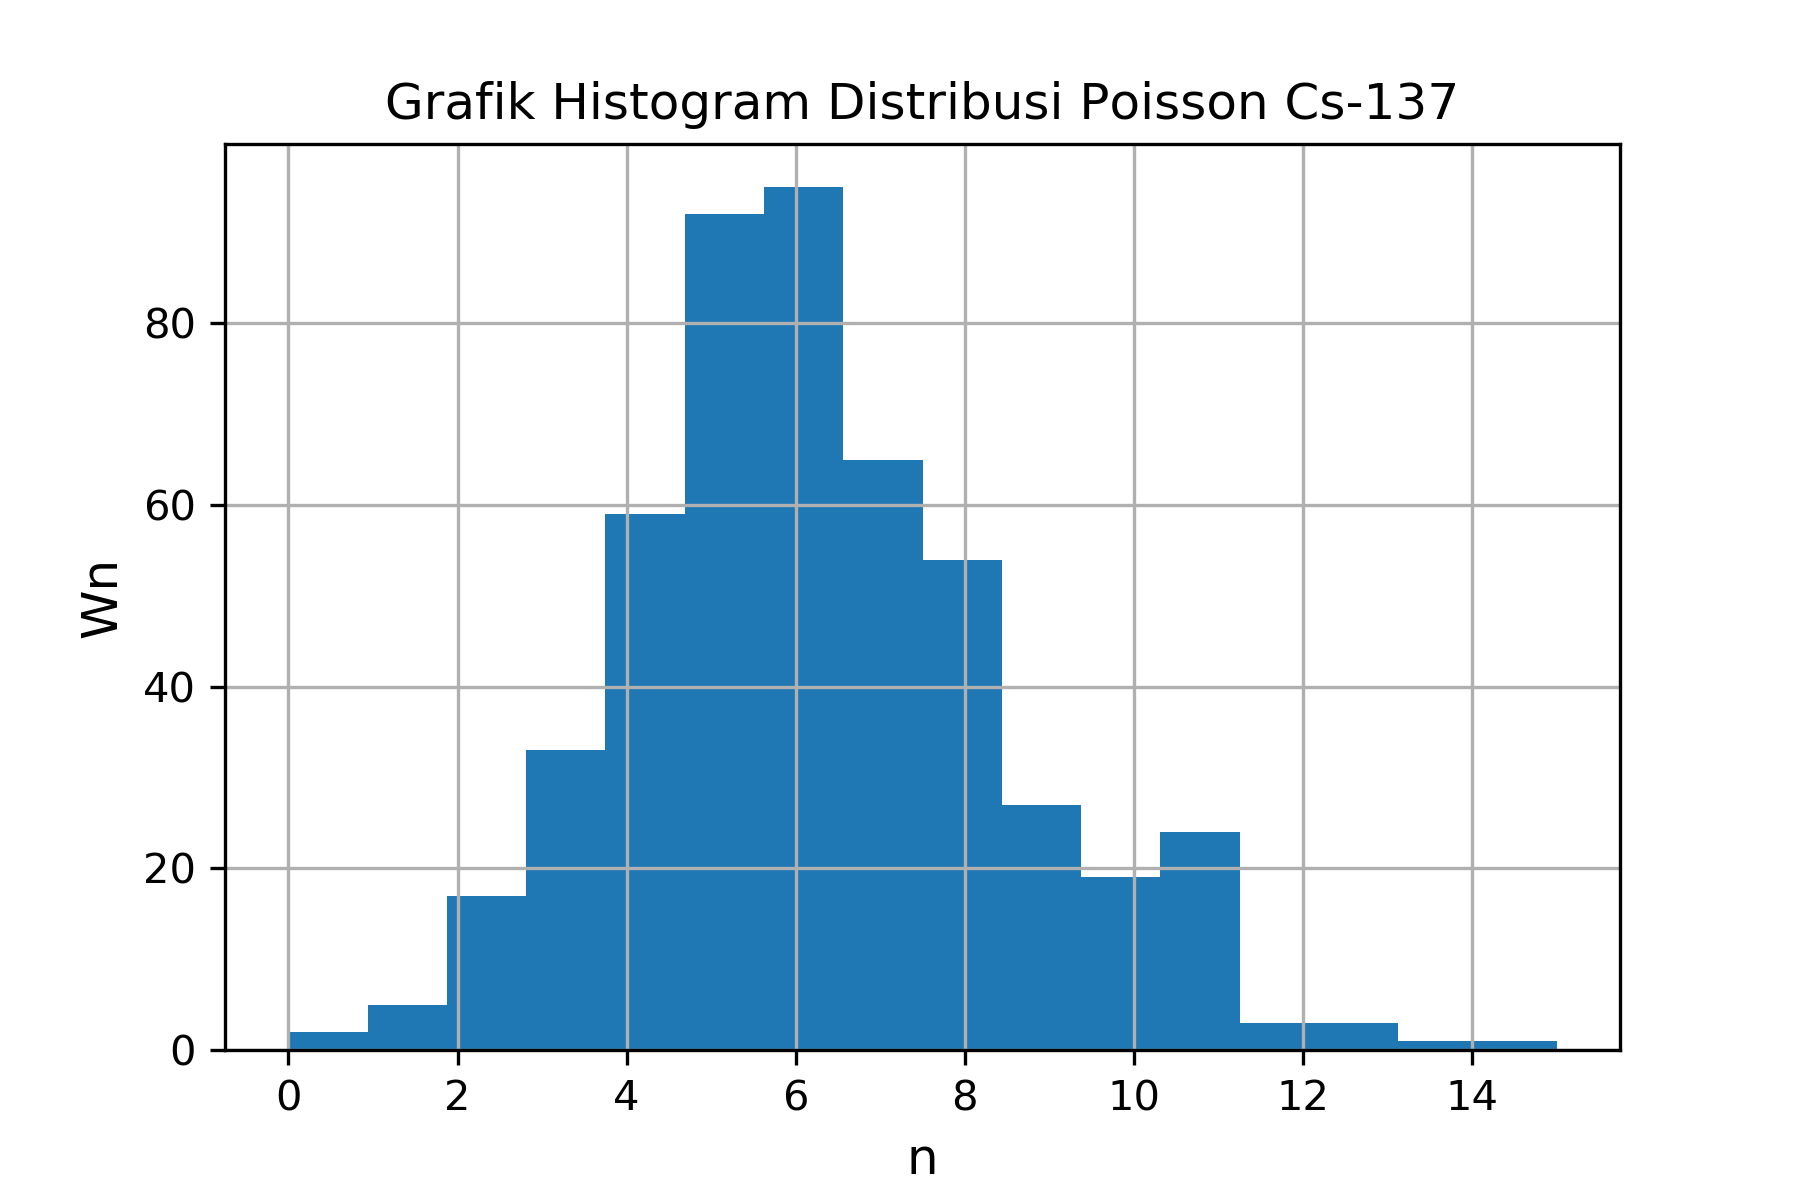
\includegraphics[width=110mm]{Data/Cs-137.png}\\
				Gambar 9. Grafik Histogram dari Preparat Cs-137.
			\end{center} 
			Nilai rata-rata standar deviasi $\sigma = \sqrt{\mu}$ berdasarkan histogram:\\
			$ \sigma = \sqrt{-(-6.13748382)} = 2.477394562842181 $\newpage
			
			\subsection{Am-241}
			Tabel Pengolahan Data:
			\begin{longtable}{@{}lllllllll@{}}
				\toprule
				No  & $n$  & $n^{2}$ & $n!$   & $h$   & $w$     & $ln(w.n!)$     & $ln^{2}(w.n!)$ & $n.ln(w.n!)$   \\ \midrule
				\endfirsthead
				%
				\endhead
				%
				\bottomrule
				\endfoot
				%
				\endlastfoot
				%
				1   & 0  & 0                    & 1     & 75  & 0.15  & -1.897119985 & 3.599064237                 & 0            \\
				2   & 1  & 1                    & 1     & 132 & 0.264 & -1.331806176 & 1.77370769                  & -1.331806176 \\
				3   & 2  & 4                    & 2     & 147 & 0.294 & -0.531028331 & 0.281991088                 & -1.062056662 \\
				4   & 3  & 9                    & 6     & 93  & 0.186 & 0.109750864  & 0.012045252                 & 0.329252592  \\
				5   & 4  & 16                   & 24    & 29  & 0.058 & 0.330741562  & 0.109389981                 & 1.322966248  \\
				6   & 5  & 25                   & 120   & 19  & 0.038 & 1.517322624  & 2.302267944                 & 7.586613118  \\
				7   & 6  & 36                   & 720   & 4   & 0.008 & 1.750937475  & 3.06578204                  & 10.50562485  \\
				8   & 8  & 64                   & 40320 & 1   & 0.002 & 4.389994804  & 19.27205438                 & 35.11995843  \\* \midrule
				$\Sigma$ & 29 & 155                  & 41194 & 500 & 1     & 4.338792837  & 30.41630261                 & 52.4705524   \\* \bottomrule
			\end{longtable}
			\hspace{-0.6cm}Koefisien Regresi, \\
			$a = -2.12815321$ \\
			$b = 0.73669029$ \\ \\
			Error,\\
			$r^{2} = 0.9645310150242827$ \\
			$r = 0.9821053991422116$ \\	\\		
			Grafik: 
			\begin{center}
				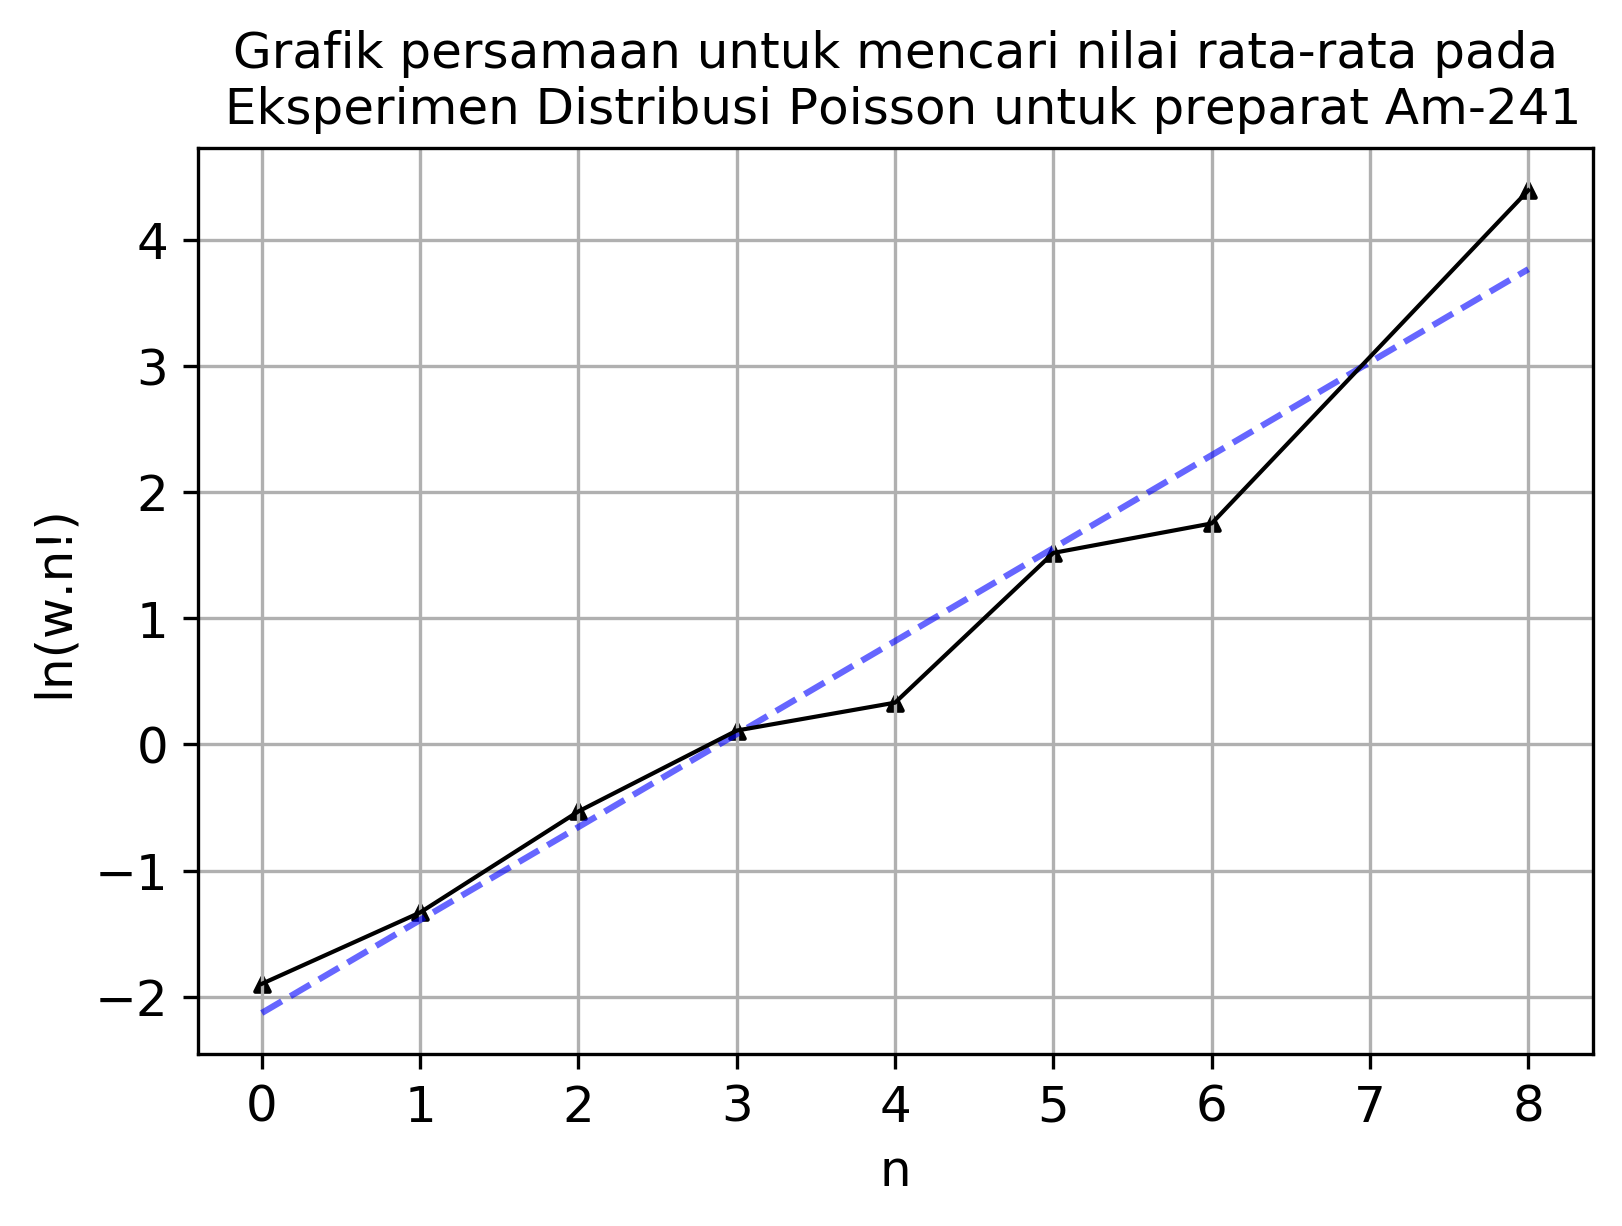
\includegraphics[width=110mm]{Data/Am-241-Graph.png}\\
				Gambar 10. Grafik Regresi Linier dari Preparat Am-241.
			\end{center} \newpage
			Grafik Histogram:
			\begin{center}
				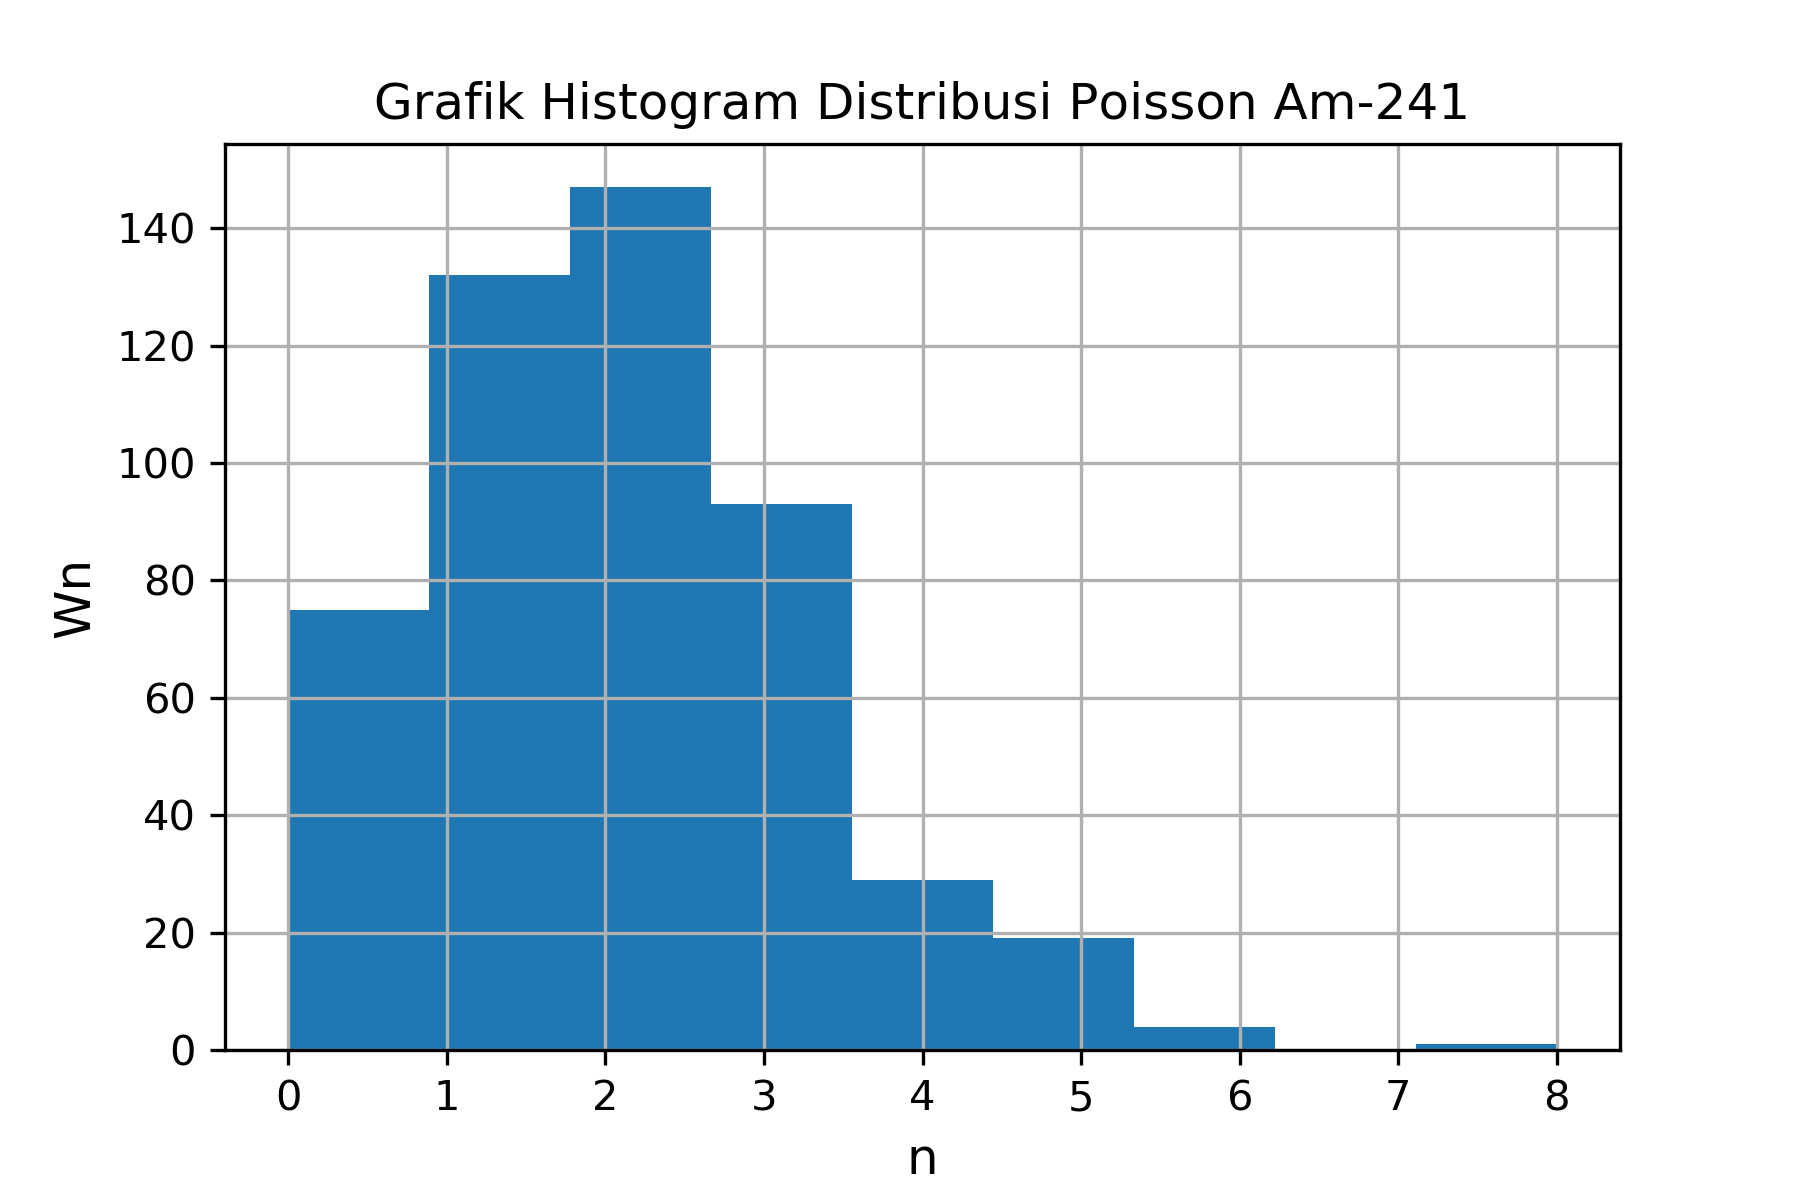
\includegraphics[width=110mm]{Data/Am-241.png}\\
				Gambar 11. Grafik Histogram dari Preparat Am-241.
			\end{center}
			Nilai rata-rata standar deviasi $\sigma = \sqrt{\mu}$ berdasarkan histogram:\\			
			$\sigma = \sqrt{-(-2.12815321)} = 1.458819114900816$
			
			\subsection{Perbandingan data antar preparat}
				\begin{longtable}{@{}llllll@{}}
					\toprule
					Preparat &
					\multicolumn{1}{c}{$a$} &
					\multicolumn{1}{c}{$b$} &
					\multicolumn{1}{c}{$r^{2}$} &
					\multicolumn{1}{c}{$r$} &
					\multicolumn{1}{c}{$\sigma$} \\* \midrule
					\endfirsthead
					%
					\endhead
					%
					\bottomrule
					\endfoot
					%
					\endlastfoot
					%
					Am-241 & -2.128  & 0.736 & 0.964 & 0.982 & 1.458 \\
					Co-60  & -1.366  & 0.303 & 0.892 & 0.944 & 1.169 \\
					Cs-137 & -6.137  & 1.812 & 0.998 & 0.999 & 2.477 \\
					Na-22  & -1.81   & 0.586 & 0.989 & 0.994 & 1.345 \\
					Sr-90  & -61.737 & 4.124 & 0.999 & 0.999 & 7.857 \\* \bottomrule
				\end{longtable}
			
	
	\section{Pembahasan}
	
		\hspace{0.35 cm} Pada praktikum kali ini, kami melakukan praktikum Distribusi Poisson secara remote (dikarenakan pandemi Covid-19) melalui TeamViewer. Praktikum kali ini dilakukan dengan mengkoneksikan komputer yang ada di lab ke alat pencacah Geiger Muller lalu mengontrolnya jarak jauh dengan menggunakan TeamViewer.
		
		\par Dengan menggunakan 5 preparat isotop radioaktif yaitu: Sr-90, Na-22, Co-60, Am-241 dan Cs-137 kita melakukan perhitungan frekuensi dari cacahan preparat radioaktif pada Geiger Muller. Sehingga, di setiap detik selama 500 detik kita dapat mengetahui jumlah cacahan dari isotop tersebut yang kemudian akan dibuat sebuah histogram dan akan diketahui jumlah frekuensinya melalui histogram tersebut
		
		\par Kemudian selanjutnya setelah dibuat histogramnya kita akan mendapatkan sebuah data yang kemudian akan diolah dengan menggunakan metode least square untuk menemukan $\mu$ nya atau nilai rata-ratanya dari frekuensi cacahan dari setiap preparat tersebut
		
		\par Setelah ditemukan $\mu$ nya atau nilai rata-ratanya, kemudian kita bandingkan dengan grafik histogram nya untuk mengetahui apakah ada kecocokan dari data yang sudah kita olah dengan data asli nya.
		
		\par Sehingga setelah diketahui $\mu$ nya kita dapat mengetahui aktivitas peluruhan preparat radioaktif dengan mengetahui rata-rata dari nilai peluruhannya per satuan detik, sehingga akan didapatkan karakteristik dari peluruhan preparat radioaktif tersebut
		
		\par Setelah itu, kita akan mengetahui berapa banyak jumlah dari preparat radioaktif tersebut yang meluruh per satuan detik selama 500 detik
		
		\par Contohnya adalah untuk preparat Na-22, kita akan mendapati nilai rata-ratanya berada di rentang n = 1.8, yang berarti isotop tersebut banyak yang meluruh di rentang n = 2 (dengan frekuensi di rentang 130-an) dengan standar deviasi nya adalah 1.34
		
		\par Kedua adalah untuk preparat Co-60, kita akan mendapati nilai rata-ratanya berada pada rentang n = 1.36, yang berarti isotop tersebut banyak yang meluruh di rentang n = 1 (dengan frekuensi di rentang 160-an) dengan standar deviasi nya adalah 1.169
		
		\par Ketiga adalah untuk preparat Sr-90, kita akan mendapat nilai rata-ratanya berada pada rentang n = 61.7, yang berarti isotop tersebut banyak yang meluruh di rentang n = 50-60 an (dengan frekuensi di rentang 10-30 an) dengan standar deviasi nya adalah 7.85
		
		\par Keempat adalah untuk preparat Cs-137, kita akan mendapat nilai rata-ratanya berada pada rentang n = 6.137, yang berarti isotop tersebut banyak yang meluruh di rentang n = 6-7 (dengan frekuensi di rentang 90-an) dengan standar deviasi nya adalah 2.47
		
		\par Kelima adalah untuk preparat Am-241, kita akan mendapat nilai rata-ratanya berada pada rentang n = 2.128, yang berarti isotop tersebut banyak yang meluruh di rentang n = 2-3 (dengan frekuensi di rentang 130-an) dengan standar deviasi nya adalah 1.458
		
		\par Sehingga inti dari praktikum ini adalah kita dapat mengetahui serta dapat membuktikan karakteristik statistik radioaktif dengan metode Distribusi Poisson dengan preparat radioaktif sebagai objek atau media nya. Serta dapat mengetahui aktifitas dari peluruhan preparat radioaktif tersebut dengan cara mengetahui berapa banyak isotop yang meluluh pada rentang waktu 500 detik dengan membaca frekuensi dari histogram dari isotop tersebut
	
	\section{Kesimpulan}
	
	1. Disini kita sudah mengetahui tentang karakteristik statistik dari peluruhan radioaktif yaitu salah satunya dengan menggunakan metode distribusi Poisson. Sebaran data nya diolah dengan menggunakan frekuensi dari histogram untuk didapati jumlah isotop radioaktif yang meluruh. \\ \\
	2. Aktifitas dari peluruhan radioaktif disini dapat diketahui dengan menggunakan metode least square untuk mendapatkan a nya dimana a adalah $\mu$ atau rata-rata isotop tersebut meluruh
		
	\begin{thebibliography}{9}
		\bibitem{modul} 
		Priambodo, dkk. 
		\textit{Modul Laporan Praktikum Jarak Jauh Eksperimen Fisika II}. 
		PLT UIN Jakarta, Jakarta, 2020.
	\end{thebibliography}
	
\end{document}